\documentclass[12pt]{article}
\usepackage{fontspec}
\usepackage{fullpage}
\usepackage{hyperref}
\hypersetup{bookmarks=true,colorlinks=true,linkcolor=red,citecolor=blue,filecolor=magenta,urlcolor=cyan}
\usepackage{amsmath}
\usepackage{amssymb}
\usepackage{mathtools}
\usepackage{unicode-math}
\usepackage{tabu}
\usepackage{longtable}
\usepackage{booktabs}
\usepackage{caption}
\usepackage{enumitem}
\usepackage{graphics}
\usepackage{filecontents}
\usepackage[backend=bibtex]{biblatex}
\usepackage{url}
\setmathfont{Latin Modern Math}
\newcommand{\gt}{\ensuremath >}
\newcommand{\lt}{\ensuremath <}
\global\tabulinesep=1mm
\newlist{symbDescription}{description}{1}
\setlist[symbDescription]{noitemsep, topsep=0pt, parsep=0pt, partopsep=0pt}
\bibliography{bibfile}
\title{Software Requirements Specification for Pendulum}
\author{Olu Owojaiye}
\begin{document}
\maketitle
\tableofcontents
\newpage
\section{Reference Material}
\label{Sec:RefMat}
This section records information for easy reference.

\subsection{Table of Units}
\label{Sec:ToU}
The unit system used throughout is SI (Système International d'Unités). In addition to the basic units, several derived units are also used. For each unit, \hyperref[Table:ToU]{Tab: ToU} lists the symbol, a description and the SI name.

\begin{longtable}{l l l}
\toprule
\textbf{Symbol} & \textbf{Description} & \textbf{SI Name}
\\
\midrule
\endhead
${{}^{\circ}}$ & angle & degree
\\
${\text{Hz}}$ & frequency & hertz
\\
${\text{kg}}$ & mass & kilogram
\\
${\text{m}}$ & length & metre
\\
${\text{N}}$ & force & newton
\\
${\text{rad}}$ & angle & radian
\\
${\text{s}}$ & time & second
\\
\bottomrule
\caption{Table of Units}
\label{Table:ToU}
\end{longtable}
\subsection{Table of Symbols}
\label{Sec:ToS}
The symbols used in this document are summarized in \hyperref[Table:ToS]{Tab: ToS} along with their units. Throughout the document, symbols in bold will represent vectors, and scalars otherwise. The symbols are listed in alphabetical order. For vector quantities, the units shown are for each component of the vector.

\begin{longtable}{l l l}
\toprule
\textbf{Symbol} & \textbf{Description} & \textbf{Units}
\\
\midrule
\endhead
${a_{\text{x}}}$ & $x$-component of acceleration & $\frac{\text{m}}{\text{s}^{2}}$
\\
${a_{\text{y}}}$ & $y$-component of acceleration & $\frac{\text{m}}{\text{s}^{2}}$
\\
$\mathbf{a}$ & Acceleration & $\frac{\text{m}}{\text{s}^{2}}$
\\
$\mathbf{F}$ & Force & ${\text{N}}$
\\
$f$ & Frequency & ${\text{Hz}}$
\\
$\mathbf{g}$ & Gravitational acceleration & $\frac{\text{m}}{\text{s}^{2}}$
\\
$\mathbf{I}$ & Moment of inertia & $\text{kg}\text{m}^{2}$
\\
$\mathbf{\hat{i}}$ & Unit Vector & --
\\
${L_{\text{rod}}}$ & Length of rod & ${\text{m}}$
\\
$m$ & Mass & ${\text{kg}}$
\\
${{p_{\text{x}}}^{\text{i}}}$ & $x$-component of initial position & ${\text{m}}$
\\
${{p_{\text{y}}}^{\text{i}}}$ & $y$-component of initial position & ${\text{m}}$
\\
$\mathbf{p}$ & Position & ${\text{m}}$
\\
$T$ & Period & ${\text{s}}$
\\
$\mathbf{T}$ & Tension & ${\text{N}}$
\\
$t$ & Time & ${\text{s}}$
\\
${v_{\text{x}}}$ & $x$-component of velocity & $\frac{\text{m}}{\text{s}}$
\\
${v_{\text{y}}}$ & $y$-component of velocity & $\frac{\text{m}}{\text{s}}$
\\
$\mathbf{v}$ & Velocity & $\frac{\text{m}}{\text{s}}$
\\
$α$ & Angular Acceleration & $\frac{\text{rad}}{\text{s}^{2}}$
\\
$θ$ & Angular Displacement & ${\text{rad}}$
\\
${θ_{i}}$ & Initial pendulum angle & ${\text{rad}}$
\\
${θ_{p}}$ & Displacement angle of pendulum & ${{}^{\circ}}$
\\
$π$ & Ratio of circumference to diameter for any circle & --
\\
$\mathbf{τ}$ & Torque & $\text{N}\text{m}$
\\
$Ω$ & Angular frequency & ${\text{s}}$
\\
$ω$ & Angular Velocity & $\frac{\text{rad}}{\text{s}}$
\\
\bottomrule
\caption{Table of Symbols}
\label{Table:ToS}
\end{longtable}
\subsection{Abbreviations and Acronyms}
\label{Sec:TAbbAcc}
\begin{longtable}{l l}
\toprule
\textbf{Abbreviation} & \textbf{Full Form}
\\
\midrule
\endhead
2D & Two-Dimensional
\\
A & Assumption
\\
DD & Data Definition
\\
GD & General Definition
\\
GS & Goal Statement
\\
IM & Instance Model
\\
PS & Physical System Description
\\
R & Requirement
\\
SRS & Software Requirements Specification
\\
TM & Theoretical Model
\\
Uncert. & Typical Uncertainty
\\
\bottomrule
\caption{Abbreviations and Acronyms}
\label{Table:TAbbAcc}
\end{longtable}
\section{Introduction}
\label{Sec:Intro}
A pendulum consists of mass attached to the end of a rod, its moving curve is highly sensitive to initial conditions Therefore, it is useful to have a program the to simulate the motion of the pendulum to exhibit the chaotic characteristics of it The program documented here is called pendulum.

The following section provides an overview of the Software Requirements Specification (SRS) for Pendulum. This section explains the purpose of this document, the scope of the requirements, the characteristics of the intended reader, and the organization of the document.

\subsection{Scope of Requirements}
\label{Sec:ReqsScope}
The scope of the requirements includes the analysis of a two-dimensional (2D) pendulum motion problem with various initial conditions..

\section{Specific System Description}
\label{Sec:SpecSystDesc}
This section first presents the problem description, which gives a high-level view of the problem to be solved. This is followed by the solution characteristics specification, which presents the assumptions, theories, and definitions that are used.

\subsection{Problem Description}
\label{Sec:ProbDesc}
A system is needed to is needed to efficiently and correctly to predict the motion pendulum.

\subsubsection{Terminology and Definitions}
\label{Sec:TermDefs}
This subsection provides a list of terms that are used in the subsequent sections and their meaning, with the purpose of reducing ambiguity and making it easier to correctly understand the requirements.

\begin{itemize}
\item{Gravity: The force that attracts one physical body with mass to another.}
\item{Cartesian coordinate system: A coordinate system that specifies each point uniquely in a plane by a set of numerical coordinates, which are the signed distances to the point from two fixed perpendicular oriented lines, measured in the same unit of length (from \cite{cartesianWiki}).}
\end{itemize}
\subsubsection{Physical System Description}
\label{Sec:PhysSyst}
The physical system of Pendulum, as shown in \hyperref[Figure:pendulum]{Fig:pendulum}, includes the following elements:

\begin{itemize}
\item[PS1:]{The rod.}
\item[PS2:]{The mass.}
\end{itemize}
\begin{figure}
\begin{center}
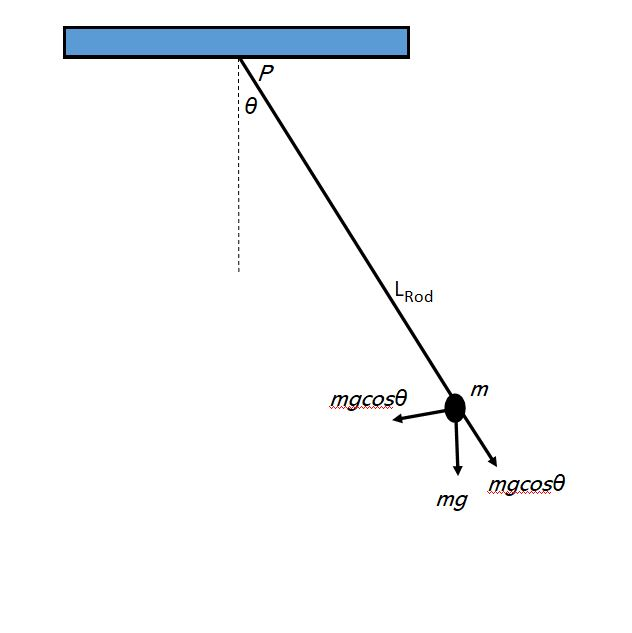
\includegraphics[width=0.7\textwidth]{../../../datafiles/DblPendulum/pendulum.jpg}
\caption{The physical system}
\label{Figure:pendulum}
\end{center}
\end{figure}
\subsubsection{Goal Statements}
\label{Sec:GoalStmt}
Given the the mass length of the rod, initial angle of the mass and the gravitational constant, the goal statements are:

\begin{itemize}
\item[Motion-of-the-mass:\phantomsection\label{motionMass}]{the Calculate the motion of the mass}
\end{itemize}
\subsection{Solution Characteristics Specification}
\label{Sec:SolCharSpec}
The instance models that govern Pendulum are presented in \hyperref[Sec:IMs]{Section: Instance Models}. The information to understand the meaning of the instance models and their derivation is also presented, so that the instance models can be verified.

\subsubsection{Assumptions}
\label{Sec:Assumps}
This section simplifies the original problem and helps in developing the theoretical models by filling in the missing information for the physical system. The assumptions refine the scope by providing more detail.

\begin{itemize}
\item[pend2DMotion:\phantomsection\label{pend2DMotion}]{The pendulum motion is two-dimensional (2D). (RefBy: \hyperref[TM:NewtonSecLawRotMot]{TM: NewtonSecLawRotMot}.)}
\item[cartCoord:\phantomsection\label{cartCoord}]{A Cartesian coordinate system is used}
\item[cartCoordRight:\phantomsection\label{cartCoordRight}]{The Cartesian coordinate system is right-handed where positive $x$-axis. and $y$-axis point right up}
\item[yAxisDir:\phantomsection\label{yAxisDir}]{The The direction of the $y$-axis is directed opposite to gravity.}
\item[startOrigin:\phantomsection\label{startOrigin}]{The pendulum is attached to the origin.}
\end{itemize}
\subsubsection{Theoretical Models}
\label{Sec:TMs}
This section focuses on the general equations and laws that Pendulum is based on.

\vspace{\baselineskip}
\noindent
\begin{minipage}{\textwidth}
\begin{tabular}{>{\raggedright}p{0.13\textwidth}>{\raggedright\arraybackslash}p{0.82\textwidth}}
\toprule \textbf{Refname} & \textbf{TM:acceleration}
\phantomsection 
\label{TM:acceleration}
\\ \midrule \\
Label & Acceleration
        
\\ \midrule \\
Equation & \begin{displaymath}
           \mathbf{a}=\frac{\,d\mathbf{v}}{\,dt}
           \end{displaymath}
\\ \midrule \\
Description & \begin{symbDescription}
              \item{$\mathbf{a}$ is the acceleration ($\frac{\text{m}}{\text{s}^{2}}$)}
              \item{$t$ is the time (${\text{s}}$)}
              \item{$\mathbf{v}$ is the velocity ($\frac{\text{m}}{\text{s}}$)}
              \end{symbDescription}
\\ \midrule \\
Source & \cite{accelerationWiki}
         
\\ \midrule \\
RefBy & 
\\ \bottomrule
\end{tabular}
\end{minipage}
\vspace{\baselineskip}
\noindent
\begin{minipage}{\textwidth}
\begin{tabular}{>{\raggedright}p{0.13\textwidth}>{\raggedright\arraybackslash}p{0.82\textwidth}}
\toprule \textbf{Refname} & \textbf{TM:velocity}
\phantomsection 
\label{TM:velocity}
\\ \midrule \\
Label & Velocity
        
\\ \midrule \\
Equation & \begin{displaymath}
           \mathbf{v}=\frac{\,d\mathbf{p}}{\,dt}
           \end{displaymath}
\\ \midrule \\
Description & \begin{symbDescription}
              \item{$\mathbf{v}$ is the velocity ($\frac{\text{m}}{\text{s}}$)}
              \item{$t$ is the time (${\text{s}}$)}
              \item{$\mathbf{p}$ is the position (${\text{m}}$)}
              \end{symbDescription}
\\ \midrule \\
Source & \cite{velocityWiki}
         
\\ \midrule \\
RefBy & 
\\ \bottomrule
\end{tabular}
\end{minipage}
\vspace{\baselineskip}
\noindent
\begin{minipage}{\textwidth}
\begin{tabular}{>{\raggedright}p{0.13\textwidth}>{\raggedright\arraybackslash}p{0.82\textwidth}}
\toprule \textbf{Refname} & \textbf{TM:NewtonSecLawMot}
\phantomsection 
\label{TM:NewtonSecLawMot}
\\ \midrule \\
Label & Newton's second law of motion
        
\\ \midrule \\
Equation & \begin{displaymath}
           \mathbf{F}=m \mathbf{a}
           \end{displaymath}
\\ \midrule \\
Description & \begin{symbDescription}
              \item{$\mathbf{F}$ is the force (${\text{N}}$)}
              \item{$m$ is the mass (${\text{kg}}$)}
              \item{$\mathbf{a}$ is the acceleration ($\frac{\text{m}}{\text{s}^{2}}$)}
              \end{symbDescription}
\\ \midrule \\
Notes & The net force $\mathbf{F}$ on a body is proportional to the acceleration $\mathbf{a}$ of the body, where $m$ denotes the mass of the body as the constant of proportionality.
        
\\ \midrule \\
Source & --
         
\\ \midrule \\
RefBy & 
\\ \bottomrule
\end{tabular}
\end{minipage}
\vspace{\baselineskip}
\noindent
\begin{minipage}{\textwidth}
\begin{tabular}{>{\raggedright}p{0.13\textwidth}>{\raggedright\arraybackslash}p{0.82\textwidth}}
\toprule \textbf{Refname} & \textbf{TM:NewtonSecLawRotMot}
\phantomsection 
\label{TM:NewtonSecLawRotMot}
\\ \midrule \\
Label & Newton's second law for rotational motion
        
\\ \midrule \\
Equation & \begin{displaymath}
           \mathbf{τ}=\mathbf{I} α
           \end{displaymath}
\\ \midrule \\
Description & \begin{symbDescription}
              \item{$\mathbf{τ}$ is the torque ($\text{N}\text{m}$)}
              \item{$\mathbf{I}$ is the moment of inertia ($\text{kg}\text{m}^{2}$)}
              \item{$α$ is the angular acceleration ($\frac{\text{rad}}{\text{s}^{2}}$)}
              \end{symbDescription}
\\ \midrule \\
Notes & The net torque $\mathbf{τ}$ on a pendulum is proportional to its angular acceleration $α$, where $\mathbf{I}$ denotes the moment of inertia of the pendulum as the constant of proportionality We also assume that pendulum motion is two-dimensional \hyperref[pend2DMotion]{A: pend2DMotion}.
        
\\ \midrule \\
Source & --
         
\\ \midrule \\
RefBy & \hyperref[IM:calOfAngularDisplacement]{IM: calOfAngularDisplacement} and \hyperref[GD:angFrequencyGD]{GD: angFrequencyGD}
        
\\ \bottomrule
\end{tabular}
\end{minipage}
\subsubsection{General Definitions}
\label{Sec:GDs}
This section collects the laws and equations that will be used to build the instance models.

\vspace{\baselineskip}
\noindent
\begin{minipage}{\textwidth}
\begin{tabular}{>{\raggedright}p{0.13\textwidth}>{\raggedright\arraybackslash}p{0.82\textwidth}}
\toprule \textbf{Refname} & \textbf{GD:velocityIX}
\phantomsection 
\label{GD:velocityIX}
\\ \midrule \\
Label & The $x$-component of velocity of the pendulum
        
\\ \midrule \\
Units & $\frac{\text{m}}{\text{s}}$
        
\\ \midrule \\
Equation & \begin{displaymath}
           {v_{\text{x}}}=ω {L_{\text{rod}}} \cos\left({θ_{p}}\right)
           \end{displaymath}
\\ \midrule \\
Description & \begin{symbDescription}
              \item{${v_{\text{x}}}$ is the $x$-component of velocity ($\frac{\text{m}}{\text{s}}$)}
              \item{$ω$ is the angular velocity ($\frac{\text{rad}}{\text{s}}$)}
              \item{${L_{\text{rod}}}$ is the length of rod (${\text{m}}$)}
              \item{${θ_{p}}$ is the displacement angle of pendulum (${{}^{\circ}}$)}
              \end{symbDescription}
\\ \midrule \\
Source & --
         
\\ \midrule \\
RefBy & 
\\ \bottomrule
\end{tabular}
\end{minipage}
\paragraph{Detailed derivation of $x$-component velocity:}
\label{GD:velocityIXDeriv}
\begin{displaymath}
{v_{\text{x}}}=ω {L_{\text{rod}}} \cos\left({θ_{p}}\right)
\end{displaymath}
\vspace{\baselineskip}
\noindent
\begin{minipage}{\textwidth}
\begin{tabular}{>{\raggedright}p{0.13\textwidth}>{\raggedright\arraybackslash}p{0.82\textwidth}}
\toprule \textbf{Refname} & \textbf{GD:velocityIY}
\phantomsection 
\label{GD:velocityIY}
\\ \midrule \\
Label & The $y$-component of velocity of the pendulum
        
\\ \midrule \\
Units & $\frac{\text{m}}{\text{s}}$
        
\\ \midrule \\
Equation & \begin{displaymath}
           {v_{\text{y}}}=ω {L_{\text{rod}}} \cos\left({θ_{p}}\right)
           \end{displaymath}
\\ \midrule \\
Description & \begin{symbDescription}
              \item{${v_{\text{y}}}$ is the $y$-component of velocity ($\frac{\text{m}}{\text{s}}$)}
              \item{$ω$ is the angular velocity ($\frac{\text{rad}}{\text{s}}$)}
              \item{${L_{\text{rod}}}$ is the length of rod (${\text{m}}$)}
              \item{${θ_{p}}$ is the displacement angle of pendulum (${{}^{\circ}}$)}
              \end{symbDescription}
\\ \midrule \\
Source & --
         
\\ \midrule \\
RefBy & 
\\ \bottomrule
\end{tabular}
\end{minipage}
\paragraph{Detailed derivation of $y$-component velocity:}
\label{GD:velocityIYDeriv}
\begin{displaymath}
{v_{\text{y}}}=ω {L_{\text{rod}}} \cos\left({θ_{p}}\right)
\end{displaymath}
\vspace{\baselineskip}
\noindent
\begin{minipage}{\textwidth}
\begin{tabular}{>{\raggedright}p{0.13\textwidth}>{\raggedright\arraybackslash}p{0.82\textwidth}}
\toprule \textbf{Refname} & \textbf{GD:accelerationIX}
\phantomsection 
\label{GD:accelerationIX}
\\ \midrule \\
Label & The $x$-component of acceleration of the pendulum
        
\\ \midrule \\
Units & $\frac{\text{m}}{\text{s}^{2}}$
        
\\ \midrule \\
Equation & \begin{displaymath}
           {a_{\text{x}}}=-ω {L_{\text{rod}}} \sin\left({θ_{p}}\right)+α {L_{\text{rod}}} \cos\left({θ_{p}}\right)
           \end{displaymath}
\\ \midrule \\
Description & \begin{symbDescription}
              \item{${a_{\text{x}}}$ is the $x$-component of acceleration ($\frac{\text{m}}{\text{s}^{2}}$)}
              \item{$ω$ is the angular velocity ($\frac{\text{rad}}{\text{s}}$)}
              \item{${L_{\text{rod}}}$ is the length of rod (${\text{m}}$)}
              \item{${θ_{p}}$ is the displacement angle of pendulum (${{}^{\circ}}$)}
              \item{$α$ is the angular acceleration ($\frac{\text{rad}}{\text{s}^{2}}$)}
              \end{symbDescription}
\\ \midrule \\
Source & --
         
\\ \midrule \\
RefBy & 
\\ \bottomrule
\end{tabular}
\end{minipage}
\paragraph{Detailed derivation of $x$-component acceleration:}
\label{GD:accelerationIXDeriv}
\begin{displaymath}
{a_{\text{x}}}=-ω {L_{\text{rod}}} \sin\left({θ_{p}}\right)+α {L_{\text{rod}}} \cos\left({θ_{p}}\right)
\end{displaymath}
\vspace{\baselineskip}
\noindent
\begin{minipage}{\textwidth}
\begin{tabular}{>{\raggedright}p{0.13\textwidth}>{\raggedright\arraybackslash}p{0.82\textwidth}}
\toprule \textbf{Refname} & \textbf{GD:accelerationIY}
\phantomsection 
\label{GD:accelerationIY}
\\ \midrule \\
Label & The $y$-component of acceleration of the pendulum
        
\\ \midrule \\
Units & $\frac{\text{m}}{\text{s}^{2}}$
        
\\ \midrule \\
Equation & \begin{displaymath}
           {a_{\text{y}}}=ω {L_{\text{rod}}} \cos\left({θ_{p}}\right)+α {L_{\text{rod}}} \sin\left({θ_{p}}\right)
           \end{displaymath}
\\ \midrule \\
Description & \begin{symbDescription}
              \item{${a_{\text{y}}}$ is the $y$-component of acceleration ($\frac{\text{m}}{\text{s}^{2}}$)}
              \item{$ω$ is the angular velocity ($\frac{\text{rad}}{\text{s}}$)}
              \item{${L_{\text{rod}}}$ is the length of rod (${\text{m}}$)}
              \item{${θ_{p}}$ is the displacement angle of pendulum (${{}^{\circ}}$)}
              \item{$α$ is the angular acceleration ($\frac{\text{rad}}{\text{s}^{2}}$)}
              \end{symbDescription}
\\ \midrule \\
Source & --
         
\\ \midrule \\
RefBy & 
\\ \bottomrule
\end{tabular}
\end{minipage}
\paragraph{Detailed derivation of $y$-component acceleration:}
\label{GD:accelerationIYDeriv}
\begin{displaymath}
{a_{\text{y}}}=ω {L_{\text{rod}}} \cos\left({θ_{p}}\right)+α {L_{\text{rod}}} \sin\left({θ_{p}}\right)
\end{displaymath}
\vspace{\baselineskip}
\noindent
\begin{minipage}{\textwidth}
\begin{tabular}{>{\raggedright}p{0.13\textwidth}>{\raggedright\arraybackslash}p{0.82\textwidth}}
\toprule \textbf{Refname} & \textbf{GD:hForceOnPendulum}
\phantomsection 
\label{GD:hForceOnPendulum}
\\ \midrule \\
Label & Horizontal force on the pendulum
        
\\ \midrule \\
Units & ${\text{N}}$
        
\\ \midrule \\
Equation & \begin{displaymath}
           \mathbf{F}=m {a_{\text{x}}}=-\mathbf{T} \sin\left({θ_{p}}\right)
           \end{displaymath}
\\ \midrule \\
Description & \begin{symbDescription}
              \item{$\mathbf{F}$ is the force (${\text{N}}$)}
              \item{$m$ is the mass (${\text{kg}}$)}
              \item{${a_{\text{x}}}$ is the $x$-component of acceleration ($\frac{\text{m}}{\text{s}^{2}}$)}
              \item{$\mathbf{T}$ is the tension (${\text{N}}$)}
              \item{${θ_{p}}$ is the displacement angle of pendulum (${{}^{\circ}}$)}
              \end{symbDescription}
\\ \midrule \\
Source & --
         
\\ \midrule \\
RefBy & 
\\ \bottomrule
\end{tabular}
\end{minipage}
\paragraph{Detailed derivation of force pendulum:}
\label{GD:hForceOnPendulumDeriv}
\begin{displaymath}
\mathbf{F}=m {a_{\text{x}}}=-\mathbf{T} \sin\left({θ_{p}}\right)
\end{displaymath}
\vspace{\baselineskip}
\noindent
\begin{minipage}{\textwidth}
\begin{tabular}{>{\raggedright}p{0.13\textwidth}>{\raggedright\arraybackslash}p{0.82\textwidth}}
\toprule \textbf{Refname} & \textbf{GD:vForceOnPendulum}
\phantomsection 
\label{GD:vForceOnPendulum}
\\ \midrule \\
Label & Vertical force on the pendulum
        
\\ \midrule \\
Units & ${\text{N}}$
        
\\ \midrule \\
Equation & \begin{displaymath}
           \mathbf{F}=m {a_{\text{y}}}=\mathbf{T} \cos\left({θ_{p}}\right)-m \mathbf{g}
           \end{displaymath}
\\ \midrule \\
Description & \begin{symbDescription}
              \item{$\mathbf{F}$ is the force (${\text{N}}$)}
              \item{$m$ is the mass (${\text{kg}}$)}
              \item{${a_{\text{y}}}$ is the $y$-component of acceleration ($\frac{\text{m}}{\text{s}^{2}}$)}
              \item{$\mathbf{T}$ is the tension (${\text{N}}$)}
              \item{${θ_{p}}$ is the displacement angle of pendulum (${{}^{\circ}}$)}
              \item{$\mathbf{g}$ is the gravitational acceleration ($\frac{\text{m}}{\text{s}^{2}}$)}
              \end{symbDescription}
\\ \midrule \\
Source & --
         
\\ \midrule \\
RefBy & 
\\ \bottomrule
\end{tabular}
\end{minipage}
\paragraph{Detailed derivation of force pendulum:}
\label{GD:vForceOnPendulumDeriv}
\begin{displaymath}
\mathbf{F}=m {a_{\text{y}}}=\mathbf{T} \cos\left({θ_{p}}\right)-m \mathbf{g}
\end{displaymath}
\vspace{\baselineskip}
\noindent
\begin{minipage}{\textwidth}
\begin{tabular}{>{\raggedright}p{0.13\textwidth}>{\raggedright\arraybackslash}p{0.82\textwidth}}
\toprule \textbf{Refname} & \textbf{GD:angFrequencyGD}
\phantomsection 
\label{GD:angFrequencyGD}
\\ \midrule \\
Label & The The angular frequency of the pendulum
        
\\ \midrule \\
Units & ${\text{s}}$
        
\\ \midrule \\
Equation & \begin{displaymath}
           Ω=\sqrt{\frac{\mathbf{g}}{{L_{\text{rod}}}}}
           \end{displaymath}
\\ \midrule \\
Description & \begin{symbDescription}
              \item{$Ω$ is the angular frequency (${\text{s}}$)}
              \item{$\mathbf{g}$ is the gravitational acceleration ($\frac{\text{m}}{\text{s}^{2}}$)}
              \item{${L_{\text{rod}}}$ is the length of rod (${\text{m}}$)}
              \end{symbDescription}
\\ \midrule \\
Notes & The torque is defined in \hyperref[TM:NewtonSecLawRotMot]{TM: NewtonSecLawRotMot} and frequency is $f$ is defined in \hyperref[DD:frequencyDD]{DD: frequencyDD}.
        
\\ \midrule \\
Source & --
         
\\ \midrule \\
RefBy & \hyperref[GD:periodPend]{GD: periodPend} and \hyperref[IM:calOfAngularDisplacement]{IM: calOfAngularDisplacement}
        
\\ \bottomrule
\end{tabular}
\end{minipage}
\paragraph{Detailed derivation of angular frequency pendulum:}
\label{GD:angFrequencyGDDeriv}
Consider the torque, on a pendulum defined in \hyperref[TM:NewtonSecLawRotMot]{TM: NewtonSecLawRotMot}, the force providing the restoring torque is the component of the the weight of the pendulum bob that acts along the arc length The the torque is the length of the string the ${L_{\text{rod}}}$ multiplied by the component of the net the force that is perpendicular to the radius of the arc. The minus sign indicates the torque acts in the opposite direction of the angular displacement:

\begin{displaymath}
\mathbf{τ}=-{L_{\text{rod}}} m \mathbf{g} \sin\left({θ_{p}}\right)
\end{displaymath}
So then

\begin{displaymath}
\mathbf{I} α=-{L_{\text{rod}}} m \mathbf{g} \sin\left({θ_{p}}\right)
\end{displaymath}
Therefore,

\begin{displaymath}
\mathbf{I} \frac{\,d\frac{\,d{θ_{p}}}{\,dt}}{\,dt}=-{L_{\text{rod}}} m \mathbf{g} \sin\left({θ_{p}}\right)
\end{displaymath}
Substituting for $\mathbf{I}$

\begin{displaymath}
m {L_{\text{rod}}}^{2} \frac{\,d\frac{\,d{θ_{p}}}{\,dt}}{\,dt}=-{L_{\text{rod}}} m \mathbf{g} \sin\left({θ_{p}}\right)
\end{displaymath}
Crossing out $m$ and ${L_{\text{rod}}}$ we have

\begin{displaymath}
\frac{\,d\frac{\,d{θ_{p}}}{\,dt}}{\,dt}=-\left(\frac{\mathbf{g}}{{L_{\text{rod}}}}\right) \sin\left({θ_{p}}\right)
\end{displaymath}
For small angles, we approximate sin ${θ_{p}}$ to ${θ_{p}}$

\begin{displaymath}
\frac{\,d\frac{\,d{θ_{p}}}{\,dt}}{\,dt}=-\left(\frac{\mathbf{g}}{{L_{\text{rod}}}}\right) {θ_{p}}
\end{displaymath}
Because this equation, has the same form as the equation for simple harmonic motion the solution is easy to find.  The angular frequency

\begin{displaymath}
Ω=\sqrt{\frac{\mathbf{g}}{{L_{\text{rod}}}}}
\end{displaymath}
\vspace{\baselineskip}
\noindent
\begin{minipage}{\textwidth}
\begin{tabular}{>{\raggedright}p{0.13\textwidth}>{\raggedright\arraybackslash}p{0.82\textwidth}}
\toprule \textbf{Refname} & \textbf{GD:periodPend}
\phantomsection 
\label{GD:periodPend}
\\ \midrule \\
Label & The period on the pendulum
        
\\ \midrule \\
Units & ${\text{s}}$
        
\\ \midrule \\
Equation & \begin{displaymath}
           T=2 π \sqrt{\frac{{L_{\text{rod}}}}{\mathbf{g}}}
           \end{displaymath}
\\ \midrule \\
Description & \begin{symbDescription}
              \item{$T$ is the period (${\text{s}}$)}
              \item{$π$ is the ratio of circumference to diameter for any circle (Unitless)}
              \item{${L_{\text{rod}}}$ is the length of rod (${\text{m}}$)}
              \item{$\mathbf{g}$ is the gravitational acceleration ($\frac{\text{m}}{\text{s}^{2}}$)}
              \end{symbDescription}
\\ \midrule \\
Notes & The frequency and period are defined in \hyperref[DD:frequencyDD]{DD: frequencyDD} \hyperref[DD:periodSHMDD]{DD: periodSHMDD} respectively
        
\\ \midrule \\
Source & --
         
\\ \midrule \\
RefBy & 
\\ \bottomrule
\end{tabular}
\end{minipage}
\paragraph{Detailed derivation of period pendulum:}
\label{GD:periodPendDeriv}
the The period of the pendulum can be defined from \hyperref[GD:angFrequencyGD]{GD: angFrequencyGD} equation

\begin{displaymath}
Ω=\sqrt{\frac{\mathbf{g}}{{L_{\text{rod}}}}}
\end{displaymath}
Therefore from the equation \hyperref[DD:angFrequencyDD]{DD: angFrequencyDD}, we have

\begin{displaymath}
T=2 π \sqrt{\frac{{L_{\text{rod}}}}{\mathbf{g}}}
\end{displaymath}
\subsubsection{Data Definitions}
\label{Sec:DDs}
This section collects and defines all the data needed to build the instance models.

\vspace{\baselineskip}
\noindent
\begin{minipage}{\textwidth}
\begin{tabular}{>{\raggedright}p{0.13\textwidth}>{\raggedright\arraybackslash}p{0.82\textwidth}}
\toprule \textbf{Refname} & \textbf{DD:positionIX}
\phantomsection 
\label{DD:positionIX}
\\ \midrule \\
Label & $x$-component of initial position
        
\\ \midrule \\
Symbol & ${{p_{\text{x}}}^{\text{i}}}$
         
\\ \midrule \\
Units & ${\text{m}}$
        
\\ \midrule \\
Equation & \begin{displaymath}
           {{p_{\text{x}}}^{\text{i}}}={L_{\text{rod}}} \sin\left({θ_{i}}\right)
           \end{displaymath}
\\ \midrule \\
Description & \begin{symbDescription}
              \item{${{p_{\text{x}}}^{\text{i}}}$ is the $x$-component of initial position (${\text{m}}$)}
              \item{${L_{\text{rod}}}$ is the length of rod (${\text{m}}$)}
              \item{${θ_{i}}$ is the initial pendulum angle (${\text{rad}}$)}
              \end{symbDescription}
\\ \midrule \\
Notes & ${{p_{\text{x}}}^{\text{i}}}$ is the horizontal position
        
        ${{p_{\text{x}}}^{\text{i}}}$ is shown in \hyperref[Figure:pendulum]{Fig:pendulum}.
        
\\ \midrule \\
Source & --
         
\\ \midrule \\
RefBy & 
\\ \bottomrule
\end{tabular}
\end{minipage}

\vspace{\baselineskip}
\noindent
\begin{minipage}{\textwidth}
\begin{tabular}{>{\raggedright}p{0.13\textwidth}>{\raggedright\arraybackslash}p{0.82\textwidth}}
\toprule \textbf{Refname} & \textbf{DD:positionIY}
\phantomsection 
\label{DD:positionIY}
\\ \midrule \\
Label & $y$-component of initial position
        
\\ \midrule \\
Symbol & ${{p_{\text{y}}}^{\text{i}}}$
         
\\ \midrule \\
Units & ${\text{m}}$
        
\\ \midrule \\
Equation & \begin{displaymath}
           {{p_{\text{y}}}^{\text{i}}}={L_{\text{rod}}} \cos\left({θ_{i}}\right)
           \end{displaymath}
\\ \midrule \\
Description & \begin{symbDescription}
              \item{${{p_{\text{y}}}^{\text{i}}}$ is the $y$-component of initial position (${\text{m}}$)}
              \item{${L_{\text{rod}}}$ is the length of rod (${\text{m}}$)}
              \item{${θ_{i}}$ is the initial pendulum angle (${\text{rad}}$)}
              \end{symbDescription}
\\ \midrule \\
Notes & ${{p_{\text{y}}}^{\text{i}}}$ is the vertical position
        
        ${{p_{\text{y}}}^{\text{i}}}$ is shown in \hyperref[Figure:pendulum]{Fig:pendulum}.
        
\\ \midrule \\
Source & --
         
\\ \midrule \\
RefBy & 
\\ \bottomrule
\end{tabular}
\end{minipage}

\vspace{\baselineskip}
\noindent
\begin{minipage}{\textwidth}
\begin{tabular}{>{\raggedright}p{0.13\textwidth}>{\raggedright\arraybackslash}p{0.82\textwidth}}
\toprule \textbf{Refname} & \textbf{DD:frequencyDD}
\phantomsection 
\label{DD:frequencyDD}
\\ \midrule \\
Label & Frequency
        
\\ \midrule \\
Symbol & $f$
         
\\ \midrule \\
Units & ${\text{Hz}}$
        
\\ \midrule \\
Equation & \begin{displaymath}
           f=\frac{1}{T}
           \end{displaymath}
\\ \midrule \\
Description & \begin{symbDescription}
              \item{$f$ is the frequency (${\text{Hz}}$)}
              \item{$T$ is the period (${\text{s}}$)}
              \end{symbDescription}
\\ \midrule \\
Notes & $f$ is the number of back and forth swings in one second
        
\\ \midrule \\
Source & --
         
\\ \midrule \\
RefBy & \hyperref[GD:periodPend]{GD: periodPend}, \hyperref[DD:periodSHMDD]{DD: periodSHMDD}, and \hyperref[GD:angFrequencyGD]{GD: angFrequencyGD}
        
\\ \bottomrule
\end{tabular}
\end{minipage}

\vspace{\baselineskip}
\noindent
\begin{minipage}{\textwidth}
\begin{tabular}{>{\raggedright}p{0.13\textwidth}>{\raggedright\arraybackslash}p{0.82\textwidth}}
\toprule \textbf{Refname} & \textbf{DD:angFrequencyDD}
\phantomsection 
\label{DD:angFrequencyDD}
\\ \midrule \\
Label & Angular frequency
        
\\ \midrule \\
Symbol & $Ω$
         
\\ \midrule \\
Units & ${\text{s}}$
        
\\ \midrule \\
Equation & \begin{displaymath}
           Ω=2 π\times\frac{1}{T}=\frac{2 π}{T}
           \end{displaymath}
\\ \midrule \\
Description & \begin{symbDescription}
              \item{$Ω$ is the angular frequency (${\text{s}}$)}
              \item{$π$ is the ratio of circumference to diameter for any circle (Unitless)}
              \item{$T$ is the period (${\text{s}}$)}
              \end{symbDescription}
\\ \midrule \\
Notes & $T$ is from \hyperref[DD:periodSHMDD]{DD: periodSHMDD}
        
\\ \midrule \\
Source & --
         
\\ \midrule \\
RefBy & \hyperref[GD:periodPend]{GD: periodPend}
        
\\ \bottomrule
\end{tabular}
\end{minipage}

\vspace{\baselineskip}
\noindent
\begin{minipage}{\textwidth}
\begin{tabular}{>{\raggedright}p{0.13\textwidth}>{\raggedright\arraybackslash}p{0.82\textwidth}}
\toprule \textbf{Refname} & \textbf{DD:periodSHMDD}
\phantomsection 
\label{DD:periodSHMDD}
\\ \midrule \\
Label & Period
        
\\ \midrule \\
Symbol & $T$
         
\\ \midrule \\
Units & ${\text{s}}$
        
\\ \midrule \\
Equation & \begin{displaymath}
           T=\frac{1}{f}
           \end{displaymath}
\\ \midrule \\
Description & \begin{symbDescription}
              \item{$T$ is the period (${\text{s}}$)}
              \item{$f$ is the frequency (${\text{Hz}}$)}
              \end{symbDescription}
\\ \midrule \\
Notes & $T$ is from \hyperref[DD:frequencyDD]{DD: frequencyDD}
        
\\ \midrule \\
Source & --
         
\\ \midrule \\
RefBy & \hyperref[GD:periodPend]{GD: periodPend} and \hyperref[DD:angFrequencyDD]{DD: angFrequencyDD}
        
\\ \bottomrule
\end{tabular}
\end{minipage}

\subsubsection{Instance Models}
\label{Sec:IMs}
This section transforms the problem defined in \hyperref[Sec:ProbDesc]{Section: Problem Description} into one which is expressed in mathematical terms. It uses concrete symbols defined in \hyperref[Sec:DDs]{Section: Data Definitions} to replace the abstract symbols in the models identified in \hyperref[Sec:TMs]{Section: Theoretical Models} and \hyperref[Sec:GDs]{Section: General Definitions}.

\vspace{\baselineskip}
\noindent
\begin{minipage}{\textwidth}
\begin{tabular}{>{\raggedright}p{0.13\textwidth}>{\raggedright\arraybackslash}p{0.82\textwidth}}
\toprule \textbf{Refname} & \textbf{IM:calOfAngularDisplacement}
\phantomsection 
\label{IM:calOfAngularDisplacement}
\\ \midrule \\
Label & Calculation of angular displacement
        
\\ \midrule \\
Input & ${L_{\text{rod}}}$, ${θ_{i}}$, $\mathbf{g}$
        
\\ \midrule \\
Output & ${θ_{p}}$
         
\\ \midrule \\
Input Constraints & \begin{displaymath}
                    {L_{\text{rod}}}\gt{}0
                    \end{displaymath}
                    \begin{displaymath}
                    {θ_{i}}\gt{}0
                    \end{displaymath}
                    \begin{displaymath}
                    \mathbf{g}\gt{}0
                    \end{displaymath}
\\ \midrule \\
Output Constraints & \begin{displaymath}
                     {θ_{p}}\gt{}0
                     \end{displaymath}
\\ \midrule \\
Equation & \begin{displaymath}
           {θ_{p}}\left(t\right)={θ_{i}} \cos\left(Ω t\right)
           \end{displaymath}
\\ \midrule \\
Description & \begin{symbDescription}
              \item{${θ_{p}}$ is the displacement angle of pendulum (${{}^{\circ}}$)}
              \item{$t$ is the time (${\text{s}}$)}
              \item{${θ_{i}}$ is the initial pendulum angle (${\text{rad}}$)}
              \item{$Ω$ is the angular frequency (${\text{s}}$)}
              \end{symbDescription}
\\ \midrule \\
Notes & The constraint ${θ_{i}}\gt{}0$ is required The. angular frequency is defined in \hyperref[GD:angFrequencyGD]{GD: angFrequencyGD}
        
\\ \midrule \\
Source & --
         
\\ \midrule \\
RefBy & \hyperref[outputValues]{FR: Output-Values} and \hyperref[calcAngPos]{FR: Calculate-Angular-Position-Of-Mass}
        
\\ \bottomrule
\end{tabular}
\end{minipage}
\paragraph{Detailed derivation of angular displacement:}
\label{IM:calOfAngularDisplacementDeriv}
When the pendulum is displaced to an initial angle and released, the pendulum swings back and forth with periodic motion By applying Newton's Second Law for Rotation in \hyperref[TM:NewtonSecLawRotMot]{TM: NewtonSecLawRotMot}, the equation of motion for the pendulum may be obtained:

\begin{displaymath}
\mathbf{τ}=\mathbf{I} α
\end{displaymath}
Where $\mathbf{τ}$ denotes the torque, $\mathbf{I}$ denotes the moment of inertia and $α$ denotes the angular acceleration This implies:

\begin{displaymath}
-m \mathbf{g} \sin\left({θ_{p}}\right) {L_{\text{rod}}}=m {L_{\text{rod}}}^{2} \frac{\,d\frac{\,d{θ_{p}}}{\,dt}}{\,dt}
\end{displaymath}
And rearranged as:

\begin{displaymath}
\frac{\,d\frac{\,d{θ_{p}}}{\,dt}}{\,dt}+\frac{\mathbf{g}}{{L_{\text{rod}}}} \sin\left({θ_{p}}\right)=0
\end{displaymath}
If the amplitude of angular displacement is small enough, we can approximate $\sin\left({θ_{p}}\right)={θ_{p}}$ for the purpose of a simple pendulum at very small angles. Then the equation of motion reduces to the equation of simple harmonic motion:

\begin{displaymath}
\frac{\,d\frac{\,d{θ_{p}}}{\,dt}}{\,dt}+\frac{\mathbf{g}}{{L_{\text{rod}}}} {θ_{p}}=0
\end{displaymath}
Thus the simple harmonic motion is:

\begin{displaymath}
{θ_{p}}\left(t\right)={θ_{i}} \cos\left(Ω t\right)
\end{displaymath}
\subsubsection{Data Constraints}
\label{Sec:DataConstraints}
\hyperref[Table:InDataConstraints]{Table:InDataConstraints} shows the data constraints on the input variables. The column for physical constraints gives the physical limitations on the range of values that can be taken by the variable. The uncertainty column provides an estimate of the confidence with which the physical quantities can be measured. This information would be part of the input if one were performing an uncertainty quantification exercise. The constraints are conservative, to give the user of the model the flexibility to experiment with unusual situations. The column of typical values is intended to provide a feel for a common scenario.

\begin{longtable}{l l l l}
\toprule
\textbf{Var} & \textbf{Physical Constraints} & \textbf{Typical Value} & \textbf{Uncert.}
\\
\midrule
\endhead
${L_{\text{rod}}}$ & ${L_{\text{rod}}}\gt{}0$ & $44.2$ ${\text{m}}$ & 10$\%$
\\
${θ_{i}}$ & ${θ_{i}}\gt{}0$ & $2.1$ ${\text{rad}}$ & 10$\%$
\\
\bottomrule
\caption{Input Data Constraints}
\label{Table:InDataConstraints}
\end{longtable}
\subsubsection{Properties of a Correct Solution}
\label{Sec:CorSolProps}
\hyperref[Table:OutDataConstraints]{Table:OutDataConstraints} shows the data constraints on the output variables. The column for physical constraints gives the physical limitations on the range of values that can be taken by the variable.

\begin{longtable}{l l}
\toprule
\textbf{Var} & \textbf{Physical Constraints}
\\
\midrule
\endhead
$α$ & $α\gt{}0$
\\
${θ_{p}}$ & ${θ_{p}}\gt{}0$
\\
\bottomrule
\caption{Output Data Constraints}
\label{Table:OutDataConstraints}
\end{longtable}
\section{Requirements}
\label{Sec:Requirements}
This section provides the functional requirements, the tasks and behaviours that the software is expected to complete, and the non-functional requirements, the qualities that the software is expected to exhibit.

\subsection{Functional Requirements}
\label{Sec:FRs}
This section provides the functional requirements, the tasks and behaviours that the software is expected to complete.

\begin{itemize}
\item[Input-Values:\phantomsection\label{inputValues}]{Input the values from \hyperref[Table:ReqInputs]{Table:ReqInputs}.}
\item[Verify-Input-Values:\phantomsection\label{verifyInptVals}]{Check the entered input values to ensure that they do not exceed the data constraints mentioned in \hyperref[Sec:DataConstraints]{Section: Data Constraints}. If any of the input values are out of bounds, an error message is displayed and the calculations stop.}
\item[Calculate-Angular-Position-Of-Mass:\phantomsection\label{calcAngPos}]{Calculate the following values: $θ$ (from \hyperref[IM:calOfAngularDisplacement]{IM: calOfAngularDisplacement}) and ${θ_{p}}$ (from \hyperref[IM:calOfAngularDisplacement]{IM: calOfAngularDisplacement}).}
\item[Output-Values:\phantomsection\label{outputValues}]{Output ${L_{\text{rod}}}$ (from \hyperref[IM:calOfAngularDisplacement]{IM: calOfAngularDisplacement}) and ${L_{\text{rod}}}$ (from \hyperref[IM:calOfAngularDisplacement]{IM: calOfAngularDisplacement}).}
\end{itemize}
\begin{longtable}{l l l}
\toprule
\textbf{Symbol} & \textbf{Description} & \textbf{Units}
\\
\midrule
\endhead
${L_{\text{rod}}}$ & Length of rod & ${\text{m}}$
\\
$m$ & Mass & ${\text{kg}}$
\\
$α$ & Angular Acceleration & $\frac{\text{rad}}{\text{s}^{2}}$
\\
${θ_{i}}$ & Initial pendulum angle & ${\text{rad}}$
\\
${θ_{p}}$ & Displacement angle of pendulum & ${{}^{\circ}}$
\\
\bottomrule
\caption{Required Inputs following \hyperref[inputValues]{FR: Input-Values}}
\label{Table:ReqInputs}
\end{longtable}
\subsection{Non-Functional Requirements}
\label{Sec:NFRs}
This section provides the non-functional requirements, the qualities that the software is expected to exhibit.

\begin{itemize}
\item[Correct:\phantomsection\label{correct}]{The outputs of the code have the properties described in \hyperref[Sec:CorSolProps]{Section: Properties of a Correct Solution}.}
\item[Portable:\phantomsection\label{portable}]{The code is able to be run in different environments.}
\end{itemize}
\section{Traceability Matrices and Graphs}
\label{Sec:TraceMatrices}
The purpose of the traceability matrices is to provide easy references on what has to be additionally modified if a certain component is changed. Every time a component is changed, the items in the column of that component that are marked with an ``X'' should be modified as well. \hyperref[Table:TraceMatAvsA]{Table:TraceMatAvsA} shows the dependencies of assumptions on the assumptions. \hyperref[Table:TraceMatAvsAll]{Table:TraceMatAvsAll} shows the dependencies of data definitions, theoretical models, general definitions, instance models, requirements, likely changes, and unlikely changes on the assumptions. \hyperref[Table:TraceMatRefvsRef]{Table:TraceMatRefvsRef} shows the dependencies of data definitions, theoretical models, general definitions, and instance models with each other. \hyperref[Table:TraceMatAllvsR]{Table:TraceMatAllvsR} shows the dependencies of requirements, goal statements on the data definitions, theoretical models, general definitions, and instance models.

\begin{longtable}{l l l l l l}
\toprule
\textbf{} & \textbf{\hyperref[pend2DMotion]{A: pend2DMotion}} & \textbf{\hyperref[cartCoord]{A: cartCoord}} & \textbf{\hyperref[cartCoordRight]{A: cartCoordRight}} & \textbf{\hyperref[yAxisDir]{A: yAxisDir}} & \textbf{\hyperref[startOrigin]{A: startOrigin}}
\\
\midrule
\endhead
\hyperref[pend2DMotion]{A: pend2DMotion} &  &  &  &  & 
\\
\hyperref[cartCoord]{A: cartCoord} &  &  &  &  & 
\\
\hyperref[cartCoordRight]{A: cartCoordRight} &  &  &  &  & 
\\
\hyperref[yAxisDir]{A: yAxisDir} &  &  &  &  & 
\\
\hyperref[startOrigin]{A: startOrigin} &  &  &  &  & 
\\
\bottomrule
\caption{Traceability Matrix Showing the Connections Between Assumptions dependence of each other.}
\label{Table:TraceMatAvsA}
\end{longtable}
\begin{longtable}{l l l l l l}
\toprule
\textbf{} & \textbf{\hyperref[pend2DMotion]{A: pend2DMotion}} & \textbf{\hyperref[cartCoord]{A: cartCoord}} & \textbf{\hyperref[cartCoordRight]{A: cartCoordRight}} & \textbf{\hyperref[yAxisDir]{A: yAxisDir}} & \textbf{\hyperref[startOrigin]{A: startOrigin}}
\\
\midrule
\endhead
\hyperref[DD:positionIX]{DD: positionIX} &  &  &  &  & 
\\
\hyperref[DD:positionIY]{DD: positionIY} &  &  &  &  & 
\\
\hyperref[DD:frequencyDD]{DD: frequencyDD} &  &  &  &  & 
\\
\hyperref[DD:angFrequencyDD]{DD: angFrequencyDD} &  &  &  &  & 
\\
\hyperref[DD:periodSHMDD]{DD: periodSHMDD} &  &  &  &  & 
\\
\hyperref[TM:acceleration]{TM: acceleration} &  &  &  &  & 
\\
\hyperref[TM:velocity]{TM: velocity} &  &  &  &  & 
\\
\hyperref[TM:NewtonSecLawMot]{TM: NewtonSecLawMot} &  &  &  &  & 
\\
\hyperref[TM:NewtonSecLawRotMot]{TM: NewtonSecLawRotMot} & X &  &  &  & 
\\
\hyperref[GD:velocityIX]{GD: velocityIX} &  &  &  &  & 
\\
\hyperref[GD:velocityIY]{GD: velocityIY} &  &  &  &  & 
\\
\hyperref[GD:accelerationIX]{GD: accelerationIX} &  &  &  &  & 
\\
\hyperref[GD:accelerationIY]{GD: accelerationIY} &  &  &  &  & 
\\
\hyperref[GD:hForceOnPendulum]{GD: hForceOnPendulum} &  &  &  &  & 
\\
\hyperref[GD:vForceOnPendulum]{GD: vForceOnPendulum} &  &  &  &  & 
\\
\hyperref[GD:angFrequencyGD]{GD: angFrequencyGD} &  &  &  &  & 
\\
\hyperref[GD:periodPend]{GD: periodPend} &  &  &  &  & 
\\
\hyperref[IM:calOfAngularDisplacement]{IM: calOfAngularDisplacement} &  &  &  &  & 
\\
\hyperref[inputValues]{FR: Input-Values} &  &  &  &  & 
\\
\hyperref[verifyInptVals]{FR: Verify-Input-Values} &  &  &  &  & 
\\
\hyperref[calcAngPos]{FR: Calculate-Angular-Position-Of-Mass} &  &  &  &  & 
\\
\hyperref[outputValues]{FR: Output-Values} &  &  &  &  & 
\\
\hyperref[correct]{NFR: Correct} &  &  &  &  & 
\\
\hyperref[portable]{NFR: Portable} &  &  &  &  & 
\\
\bottomrule
\caption{Traceability Matrix Showing the Connections Between Assumptions and Other Items}
\label{Table:TraceMatAvsAll}
\end{longtable}
\begin{longtable}{l l l l l l l l l l l l l l l l l l l}
\toprule
\textbf{} & \textbf{\hyperref[DD:positionIX]{DD: positionIX}} & \textbf{\hyperref[DD:positionIY]{DD: positionIY}} & \textbf{\hyperref[DD:frequencyDD]{DD: frequencyDD}} & \textbf{\hyperref[DD:angFrequencyDD]{DD: angFrequencyDD}} & \textbf{\hyperref[DD:periodSHMDD]{DD: periodSHMDD}} & \textbf{\hyperref[TM:acceleration]{TM: acceleration}} & \textbf{\hyperref[TM:velocity]{TM: velocity}} & \textbf{\hyperref[TM:NewtonSecLawMot]{TM: NewtonSecLawMot}} & \textbf{\hyperref[TM:NewtonSecLawRotMot]{TM: NewtonSecLawRotMot}} & \textbf{\hyperref[GD:velocityIX]{GD: velocityIX}} & \textbf{\hyperref[GD:velocityIY]{GD: velocityIY}} & \textbf{\hyperref[GD:accelerationIX]{GD: accelerationIX}} & \textbf{\hyperref[GD:accelerationIY]{GD: accelerationIY}} & \textbf{\hyperref[GD:hForceOnPendulum]{GD: hForceOnPendulum}} & \textbf{\hyperref[GD:vForceOnPendulum]{GD: vForceOnPendulum}} & \textbf{\hyperref[GD:angFrequencyGD]{GD: angFrequencyGD}} & \textbf{\hyperref[GD:periodPend]{GD: periodPend}} & \textbf{\hyperref[IM:calOfAngularDisplacement]{IM: calOfAngularDisplacement}}
\\
\midrule
\endhead
\hyperref[DD:positionIX]{DD: positionIX} &  &  &  &  &  &  &  &  &  &  &  &  &  &  &  &  &  & 
\\
\hyperref[DD:positionIY]{DD: positionIY} &  &  &  &  &  &  &  &  &  &  &  &  &  &  &  &  &  & 
\\
\hyperref[DD:frequencyDD]{DD: frequencyDD} &  &  &  &  &  &  &  &  &  &  &  &  &  &  &  &  &  & 
\\
\hyperref[DD:angFrequencyDD]{DD: angFrequencyDD} &  &  &  &  & X &  &  &  &  &  &  &  &  &  &  &  &  & 
\\
\hyperref[DD:periodSHMDD]{DD: periodSHMDD} &  &  & X &  &  &  &  &  &  &  &  &  &  &  &  &  &  & 
\\
\hyperref[TM:acceleration]{TM: acceleration} &  &  &  &  &  &  &  &  &  &  &  &  &  &  &  &  &  & 
\\
\hyperref[TM:velocity]{TM: velocity} &  &  &  &  &  &  &  &  &  &  &  &  &  &  &  &  &  & 
\\
\hyperref[TM:NewtonSecLawMot]{TM: NewtonSecLawMot} &  &  &  &  &  &  &  &  &  &  &  &  &  &  &  &  &  & 
\\
\hyperref[TM:NewtonSecLawRotMot]{TM: NewtonSecLawRotMot} &  &  &  &  &  &  &  &  &  &  &  &  &  &  &  &  &  & 
\\
\hyperref[GD:velocityIX]{GD: velocityIX} &  &  &  &  &  &  &  &  &  &  &  &  &  &  &  &  &  & 
\\
\hyperref[GD:velocityIY]{GD: velocityIY} &  &  &  &  &  &  &  &  &  &  &  &  &  &  &  &  &  & 
\\
\hyperref[GD:accelerationIX]{GD: accelerationIX} &  &  &  &  &  &  &  &  &  &  &  &  &  &  &  &  &  & 
\\
\hyperref[GD:accelerationIY]{GD: accelerationIY} &  &  &  &  &  &  &  &  &  &  &  &  &  &  &  &  &  & 
\\
\hyperref[GD:hForceOnPendulum]{GD: hForceOnPendulum} &  &  &  &  &  &  &  &  &  &  &  &  &  &  &  &  &  & 
\\
\hyperref[GD:vForceOnPendulum]{GD: vForceOnPendulum} &  &  &  &  &  &  &  &  &  &  &  &  &  &  &  &  &  & 
\\
\hyperref[GD:angFrequencyGD]{GD: angFrequencyGD} &  &  & X &  &  &  &  &  & X &  &  &  &  &  &  &  &  & 
\\
\hyperref[GD:periodPend]{GD: periodPend} &  &  & X & X & X &  &  &  &  &  &  &  &  &  &  & X &  & 
\\
\hyperref[IM:calOfAngularDisplacement]{IM: calOfAngularDisplacement} &  &  &  &  &  &  &  &  & X &  &  &  &  &  &  & X &  & 
\\
\bottomrule
\caption{Traceability Matrix Showing the Connections Between Items and Other Sections}
\label{Table:TraceMatRefvsRef}
\end{longtable}
\begin{longtable}{l l l l l l l l l l l l l l l l l l l l l l l l l}
\toprule
\textbf{} & \textbf{\hyperref[DD:positionIX]{DD: positionIX}} & \textbf{\hyperref[DD:positionIY]{DD: positionIY}} & \textbf{\hyperref[DD:frequencyDD]{DD: frequencyDD}} & \textbf{\hyperref[DD:angFrequencyDD]{DD: angFrequencyDD}} & \textbf{\hyperref[DD:periodSHMDD]{DD: periodSHMDD}} & \textbf{\hyperref[TM:acceleration]{TM: acceleration}} & \textbf{\hyperref[TM:velocity]{TM: velocity}} & \textbf{\hyperref[TM:NewtonSecLawMot]{TM: NewtonSecLawMot}} & \textbf{\hyperref[TM:NewtonSecLawRotMot]{TM: NewtonSecLawRotMot}} & \textbf{\hyperref[GD:velocityIX]{GD: velocityIX}} & \textbf{\hyperref[GD:velocityIY]{GD: velocityIY}} & \textbf{\hyperref[GD:accelerationIX]{GD: accelerationIX}} & \textbf{\hyperref[GD:accelerationIY]{GD: accelerationIY}} & \textbf{\hyperref[GD:hForceOnPendulum]{GD: hForceOnPendulum}} & \textbf{\hyperref[GD:vForceOnPendulum]{GD: vForceOnPendulum}} & \textbf{\hyperref[GD:angFrequencyGD]{GD: angFrequencyGD}} & \textbf{\hyperref[GD:periodPend]{GD: periodPend}} & \textbf{\hyperref[IM:calOfAngularDisplacement]{IM: calOfAngularDisplacement}} & \textbf{\hyperref[inputValues]{FR: Input-Values}} & \textbf{\hyperref[verifyInptVals]{FR: Verify-Input-Values}} & \textbf{\hyperref[calcAngPos]{FR: Calculate-Angular-Position-Of-Mass}} & \textbf{\hyperref[outputValues]{FR: Output-Values}} & \textbf{\hyperref[correct]{NFR: Correct}} & \textbf{\hyperref[portable]{NFR: Portable}}
\\
\midrule
\endhead
\hyperref[motionMass]{GS: Motion-of-the-mass} &  &  &  &  &  &  &  &  &  &  &  &  &  &  &  &  &  &  &  &  &  &  &  & 
\\
\hyperref[inputValues]{FR: Input-Values} &  &  &  &  &  &  &  &  &  &  &  &  &  &  &  &  &  &  &  &  &  &  &  & 
\\
\hyperref[verifyInptVals]{FR: Verify-Input-Values} &  &  &  &  &  &  &  &  &  &  &  &  &  &  &  &  &  &  &  &  &  &  &  & 
\\
\hyperref[calcAngPos]{FR: Calculate-Angular-Position-Of-Mass} &  &  &  &  &  &  &  &  &  &  &  &  &  &  &  &  &  & X &  &  &  &  &  & 
\\
\hyperref[outputValues]{FR: Output-Values} &  &  &  &  &  &  &  &  &  &  &  &  &  &  &  &  &  & X &  &  &  &  &  & 
\\
\hyperref[correct]{NFR: Correct} &  &  &  &  &  &  &  &  &  &  &  &  &  &  &  &  &  &  &  &  &  &  &  & 
\\
\hyperref[portable]{NFR: Portable} &  &  &  &  &  &  &  &  &  &  &  &  &  &  &  &  &  &  &  &  &  &  &  & 
\\
\bottomrule
\caption{Traceability Matrix Showing the Connections Between Requirements, Goal Statements and Other Items}
\label{Table:TraceMatAllvsR}
\end{longtable}
\section{Values of Auxiliary Constants}
\label{Sec:AuxConstants}
There are no auxiliary constants.

\section{References}
\label{Sec:References}
\begin{filecontents*}{bibfile.bib}
@book{hibbeler2004,
author={Hibbeler, R. C.},
title={Engineering Mechanics: Dynamics},
publisher={Pearson Prentice Hall},
year={2004}}
@misc{accelerationWiki,
author={Wikipedia Contributors},
title={Acceleration},
howpublished={\url{https://en.wikipedia.org/wiki/Acceleration}},
month=jun,
year={2019}}
@misc{cartesianWiki,
author={Wikipedia Contributors},
title={Cartesian coordinate system},
howpublished={\url{https://en.wikipedia.org/wiki/Cartesian\_coordinate\_system}},
month=jun,
year={2019}}
@misc{velocityWiki,
author={Wikipedia Contributors},
title={Velocity},
howpublished={\url{https://en.wikipedia.org/wiki/Velocity}},
month=jun,
year={2019}}
\end{filecontents*}
\nocite{*}
\bibstyle{ieeetr}
\printbibliography[heading=none]
\end{document}
